\documentclass[14pt,a4paper]{report}  %紙張設定

\usepackage{xeCJK} %中文字體模組
%\setCJKmainfont{標楷體} %中文字體
\setCJKmainfont{MoeStandardKai.ttf}
%\newfontfamily\sectionef{Times New Roman}%設定英文字體
\newfontfamily\sectionef{Nimbus Roman}
\usepackage{amsmath,amssymb} %數學公式、符號
\usepackage{amsfonts} %數學簍空的英文字
\usepackage{graphicx,subfigure} %圖形
\usepackage{type1cm} %調整字體絕對大小
\usepackage{textpos} %設定文字絕對位置
\usepackage[top=2.5truecm,bottom=2.5truecm,
left=3truecm,right=2.5truecm]{geometry}
\usepackage{titlesec} %目錄標題設定模組
\usepackage{titletoc} %目錄內容設定模組
\usepackage{textcomp} %表格設定模組
\usepackage{caption} %圖片標題設定
\usepackage{CJK} %中文模組
\usepackage{CJKnumb} %中文數字模組
%\usepackage{wallpaper} %浮水印
\usepackage{float}
\usepackage{enumerate}
\usepackage{listings} %引用程式碼
\usepackage{setspace}
\graphicspath{{img/}} %圖片預設讀取路徑
\renewcommand{\figurename}{\large 圖} %更改圖片標題名稱


%=------------------更改標題內容----------------------=%
\titleformat{\chapter}[hang]{\center\sectionef\fontsize{20pt}{1pt}\bfseries}{}{}{}
\titleformat{\section}[hang]{\sectionef\fontsize{18pt}{2.5pt}\bfseries}{{\thesection}}{0.5em}{}[]
\titleformat{\subsection}[hang]{\sectionef\fontsize{18pt}{2.5pt}\bfseries}{{\thesubsection}}{1em}{}[]

%=------------------更改目錄內容----------------------=%
\titlecontents{chapter}[-5em]{}{\sectionef\fontsize{16pt}{3pt}\bfseries\makebox[2.5em][l]{\CJKmainfont}}{}{\titlerule*[0.7pc]{.}\contentspage}
\titlecontents{section}[3em]{}{\sectionef\fontsize{15pt}{3pt}\mdseries\makebox[1.5em][l]{\thecontentslabel}}{}{\titlerule*[0.7pc]{.}\contentspage}
\titlecontents{subsection}[5em]{}{\sectionef\fontsize{15pt}{3pt}\mdseries\makebox[2.5em][l]{{\thecontentslabel}}}{}{\titlerule*[0.7pc]{.}\contentspage}

%=------------------更改圖目錄內容----------------------=%
\titlecontents{figure}[1em]{}{\sectionef\fontsize{16pt}{3pt}\mdseries\makebox[1.5em][l]圖{\thecontentslabel}\quad}{}{\titlerule*[0.7pc]{.}\contentspage}

%=------------------章節間距----------------------=%
\titlespacing*{\chapter} {0pt}{0pt}{18pt}
\titlespacing*{\section} {0pt}{12pt}{6pt}
\titlespacing*{\subsection} {0pt}{6pt}{6pt}

%=------------------文件----------------------=%
\begin{document}
\begin{titlepage}
%\maketitle %文件資料
\begin{center}
\makebox[1.5\width][s] %設定文字盒子[方框寬度的1.5倍寬][對其方式為文字平均分分布於方框中]
{\fontsize{24pt}{2.5pt}國立虎尾科技大學}\\[15pt] %\\距離下方5pt
%{\ten{National Formosa University}}\\[20pt]
\makebox[1.2\width][s]
{\fontsize{24pt}{2.5pt}機械設計工程系暨精密機械工程科}\\[15pt]
%{\ten{Department of Mechanical Design Engineering \& Department of Junior Precision Mechanical Engineering}}\\[20pt]
\makebox[1.5\width][s]
{\fontsize{24pt}{2.5pt}專題製作報告}\\[120pt]
%{\ten{Project\quad Report}}\\[80pt]
{\fontsize{24pt}{2.5pt}網際內容管理系統}\\
%{\ten{Application of Web-based Content Management Systems}\\[5pt]
{\fontsize{24pt}{2.5pt}在精密機械工程教學與研究上的應用}\\[50pt]
%{\ten{in Teaching and Research of Precision Mechanical Engineering}}
{\fontsize{18pt}{2.5pt}\bf Application of Web-based Content Management Systems in Teaching and Research of Precision Mechanical Engineering}
\end{center}
\begin{flushleft}
\begin{LARGE}
\vspace{5em}
\hspace{32mm}\makebox[5cm][s]%空白距離32mm,設定文字盒子[寬度為5cm][對其方式為文字平均分分布於方框中]
{指導教授:\quad 嚴\quad 家\quad 銘\quad 老\quad 師}\\[6pt]
\hspace{32mm}\makebox[5cm][s]
{班\qquad 級:\quad 五\quad 精\quad 四\quad 甲}\\[6pt]
\hspace{32mm}\makebox[5cm][s]
{學\qquad 生:\quad 郭\qquad \quad 樺\quad(50733105)}\\[6pt]
\hspace{32mm}\makebox[5cm][s]
{\hspace{36.5mm}高\quad 沁\quad 安\quad(50733144)}\\[6pt]
\hspace{32mm}\makebox[5cm][s]
{\hspace{36.5mm}林\quad 冠\quad 澔\quad(50733146)}\\[6pt]
\hspace{32mm}\makebox[5cm][s]
{\hspace{36.5mm}林\quad 侑\quad 昌\quad(50733152)}\\[6pt]
\end{LARGE}
\end{flushleft}
\vspace{6em}
\fontsize{18pt}{2pt}\selectfont\centerline{\makebox[\width][s]
{中華民國\hspace{3em} 
110 \quad 年\quad 6\quad 月}}
\end{titlepage}

%=------------------專題製作合可證明----------------------=%
\newpage
{\renewcommand\baselinestretch{1.2}\selectfont %設定以下行距
{\begin{center}
{\fontsize{20pt}{2.5pt} {國立虎尾科技大學}\\[10pt]{機械設計工程系暨精密機械工程科}\\[10pt]{學生專題製作合格認可證明}\\
\\[40pt]
\par}
\end{center}}
{\begin{textblock}{60}(1.85,1.5)
\noindent \fontsize{16pt}{16pt}\selectfont 專題製作學生\enspace:\quad
{\begin{minipage}[t]{10em}\underline{五精四甲\enspace 50733105\enspace 郭\quad 樺}\\ \underline{五精四甲\enspace 50733144\enspace 高沁安}\\ \underline{五精四甲\enspace 50733146\enspace 林冠澔}\\ \underline{五精四甲\enspace 50733152\enspace 林侑昌} %下劃線符號指令
\end{minipage}}
\par} %結束指定行距
{\renewcommand\baselinestretch{1}\selectfont %設定以下行距
{\begin{textblock}{35}(1.8,4)
\noindent \fontsize{16pt}{16pt}\selectfont 專題製作題目\enspace: \quad
{\begin{minipage}[t]{12em}{網際內容管理系統在精密機械工程教學與研究上的應用}
\end{minipage}}
%\quad 網際內容管理系統在精密機械\\工程教學與研究上的應用
%\noindent \fontsize{16pt}{16pt}\selectfont 經評量合格,特此證明
\hspace*{\fill} \\
\hspace*{\fill} \\
\hspace*{\fill} \\
\hspace*{\fill} \\
\hspace*{\fill} \\
\hspace*{\fill} \\
\noindent \fontsize{16pt}{16pt} \makebox[6em][s]{評審委員}\enspace:\quad
{\begin{minipage}[t]{6em} \underline{            }\\[16pt] \underline{            }\\[16pt] \underline{            }\\[16pt] \underline{            }
\end{minipage}}
\end{textblock}}
{\begin{textblock}{10}(1.8,9)
{\begin{flushleft}
\fontsize{16pt}{16pt}\selectfont \makebox[6em][s]{指導老師}\enspace:\quad \underline{            }\\[10pt]
\fontsize{16pt}{16pt}\selectfont \makebox[6em][s]{系主任}\enspace:\quad \underline{            }\\
\hspace*{\fill} \\
\hspace*{\fill} \\
\hspace*{\fill} \\
\fontsize{16pt}{16pt}\selectfont \makebox[6em][s]{中華民國}\hspace{4em}年\hspace{4em}月\hspace{4em}日

\end{flushleft}}
\end{textblock}}
\end{textblock}}
\par} %結束指定行距

%=------------------摘要----------------------=%
%\newpage
%input{abstract-c.tex}

%=------------------Abstract----------------------=%
%\newpage
%\chapter{Abstract}
\renewcommand{\baselinestretch}{10} %設定行距
\par
\renewcommand{\baselinestretch}{1} %設定行距
\twelve \qquad 
\par

%=------------------致謝----------------------=%
%\newpage
%\chapter{致謝}
\renewcommand{\baselinestretch}{10} %設定行距
\par
\renewcommand{\baselinestretch}{1} %設定行距
\twelve \qquad 
\par

%=------------------目錄----------------------=%
%\newpage
%\pagenumbering{empty}%隱藏頁數
\renewcommand{\contentsname}{\centerline{\fontsize{18pt}{\baselineskip}\selectfont\textbf{目\quad 錄}}}
\begin{spacing}{2.5}
\tableofcontents %目錄產生
\end{spacing}
\par

%=------------------圖目錄----------------------=%
%\newpage
%\pagenumbering{empty}%隱藏頁數
\renewcommand{\listfigurename}{\centerline{\fontsize{18pt}{\baselineskip}\selectfont\textbf{圖\quad 目\quad 錄 }}}
\begin{spacing}{2.5}
\listoffigures %圖目錄產生
\end{spacing}


%=------------------前言----------------------=%
\newpage
\chapter{前言}
\renewcommand{\baselinestretch}{10} %設定行距
\section{研究動機}
\par
\renewcommand{\baselinestretch}{2} %設定行距
\twelve \qquad 我們是以教學與研究歷程的重要性作為研究動機,因為我們發現很多學術上的研究流程不夠詳細,導致後者無法完全得知這些專案的過程是如何進行,造成他們無法順利地接手,甚至重頭開始進行,所以我們希望不只提供學生在學習與研究流程能夠不只留下具體成果,也能有效呈現更細部的歷程與資訊,以作為學習與研究更有力的佐證資料。
\par
\renewcommand{\baselinestretch}{20} %設定行距
\section{製作目的}
\par
\renewcommand{\baselinestretch}{1} %設定行距
\twelve \qquad 目的分為兩部分:
\begin{enumerate}
\item 探討如何利用 Fossil SCM 虛擬與實體伺服器,讓五專精密機械工程科所有相關師生包含已經畢業的校友,得以透過 @gmail 帳號登入,並在網際內容管理系統中進行知識管理與互動,擬藉此提升課程教學與專題研究效益。
\item 允許使用者透過學校配發的 @gm 登入後,有權限在伺服器上自行建立獨立的倉儲系統並且自行管理。
\end{enumerate}
\par
\renewcommand{\baselinestretch}{20} %設定行距
\section{未來展望}
\par
\renewcommand{\baselinestretch}{1} %設定行距
\twelve \qquad 此專題希望用戶能利用架設的分散式版次管理系統在各別的倉儲或社群進行社會化共同項目開發與資訊交流等,包括允許使用者追蹤其他使用者、組織、軟體庫的相關資訊,對開發項目進行評論且改動等。
\par}

%=------------------提升教學品質----------------------=%
%\newpage
%\chapter{網際內容如何提升教學品質}
\renewcommand{\baselinestretch}{10} %設定行距
%\section{前言}
\par
\renewcommand{\baselinestretch}{2} %設定行距
\twelve 從教學與研究歷程的重要性作為研究動機,希望不只提供學生在學習與研究流程能夠不只留下具體成果,也能有效呈現更細部的歷程資料,以作為學習與研究更有力的佐證資料。
\par

\renewcommand{\baselinestretch}{20} %設定行距
\section{費曼學習法}
\par
\renewcommand{\baselinestretch}{1} %設定行距
\twelve 研究顯示,人類的學習型態分為以下兩種,而當兩種行為同時進行時,能使學習成效大幅提升。
\begin{itemize}
	\item 主動學習
	\item 被動學習
\end{itemize}
\par
\renewcommand{\baselinestretch}{1} %設定行距
\twelve 何謂被動學習? 老師傳播知識,而學生進行吸收,或是透過網路及大眾媒體接收資訊,這些都是常見的被動學習,也是人類大部分獲得知識的渠道。
\par
\renewcommand{\baselinestretch}{1} %設定行距
\twelve 主動學習則是,學習者在接收到資訊後,主動並有意識的思考,在腦中形成一個自己理解方式或產生其他疑問,再去透過尋找資料,主動研究,或是與人討論甚至透過教學等行動進行的學習方式。
\\
\par

\renewcommand{\baselinestretch}{20} %設定行距
\subsection{從費曼學習法的角度觀看}
\par
\renewcommand{\baselinestretch}{1} %設定行距
\twelve 現今華人地區的教學方式,最大的特徵就是「填鴨式」教育。華人的教師認為,他們在課堂上不得不放慢他們習慣的教學進度,因為學生聽不懂也記不住,他們期待學生將聽到的知識記下來,然後就可以應用,可是當這種教育放在國外會發現,很多學生都做不到這一點,他們總是要問「為什麼?,例如:為什麼這條輔助線要劃在這裡,為什麼這道題要這麼算......中方老師的教法,在某種程度上,其實就是一種「填鴨式」,你不需要了解這算法背後的原理,你只需要能夠處理這種算法,學會它並且應用它。可是外國學生對此接受無能,他們沒這個習慣,要在短時間內被「填入」這麼多知識,於是課堂進度被拖慢了。
\par

\renewcommand{\baselinestretch}{20} %設定行距
\subsection{費曼學習法的研究成效}
\par
\renewcommand{\baselinestretch}{1} %設定行距
\twelve 會發現我們的學生會習慣於「接受填鴨」這種僵化的方式去被動學習;反觀外國的學生,在他們的教學體制下,學生會敢於問「為甚麼?」,當他們問出這個問題,並且開始和老師同學討論時,學生就會處於主動學習的狀態了,這時他們的學習效果會大幅提升。\\
\par
\renewcommand{\baselinestretch}{1} %設定行距
\twelve 在生活環境中會有大量的資訊塞入我們的腦中,但是這些資訊屬於被動學習,實際吸收進去的只有不到30\%,而透過研究、紀錄、寫心得甚至教學的方式,與我們腦中的被動資訊相輔相成,可以使資訊吸收的效益增加到80\%~90\%。
\\
\par
\renewcommand{\baselinestretch}{1} %設定行距
\twelve 如(圖\ref{fig.學習金字塔})
\begin{enumerate}
	\item 講課: 授課只是純粹在學生面前說話,不涉及學生的參與,學生只能牢記當中5\% 的知識。
	\item 閱讀: 授課方式增加一個簡報或是參考資料,讓同學邊看邊閱讀,就會稍稍提高到10\%。
	\item 視聽: 授課時播放相關知識的影片,學生的知識牢記率,就會提升到20\%。
	\item 示範: 很多科學科為什麼會特別喜歡做實驗,因為示範比純粹說話好一點,學生的知識牢記率可以提升到30\%。
	\item 小組討論: 當學生直接參與整個學習過程,知識牢記率會大大提升。例如,小組活動,因為這樣就能夠將知識內化成自身的想法,然後再表達出來,這麼知識牢記率就能提升到50\%。
	\item 實踐: 實際動手比看著老師示範好,很多時候科學實驗是老師先做,然後學生再做實際動手,這樣知識牢記率就能提升到80\%。
	\item 教其他人: 最好的知識牢記方法是教其他人,原因是你內化再表達的時候,你會透過不斷教人而增強了對知識的記憶,而達到真正了解、完全吸收資訊。
\end{enumerate}
\par
\renewcommand{\baselinestretch}{1.7} %設定行距
\begin{figure}[hbt!]
\begin{center}
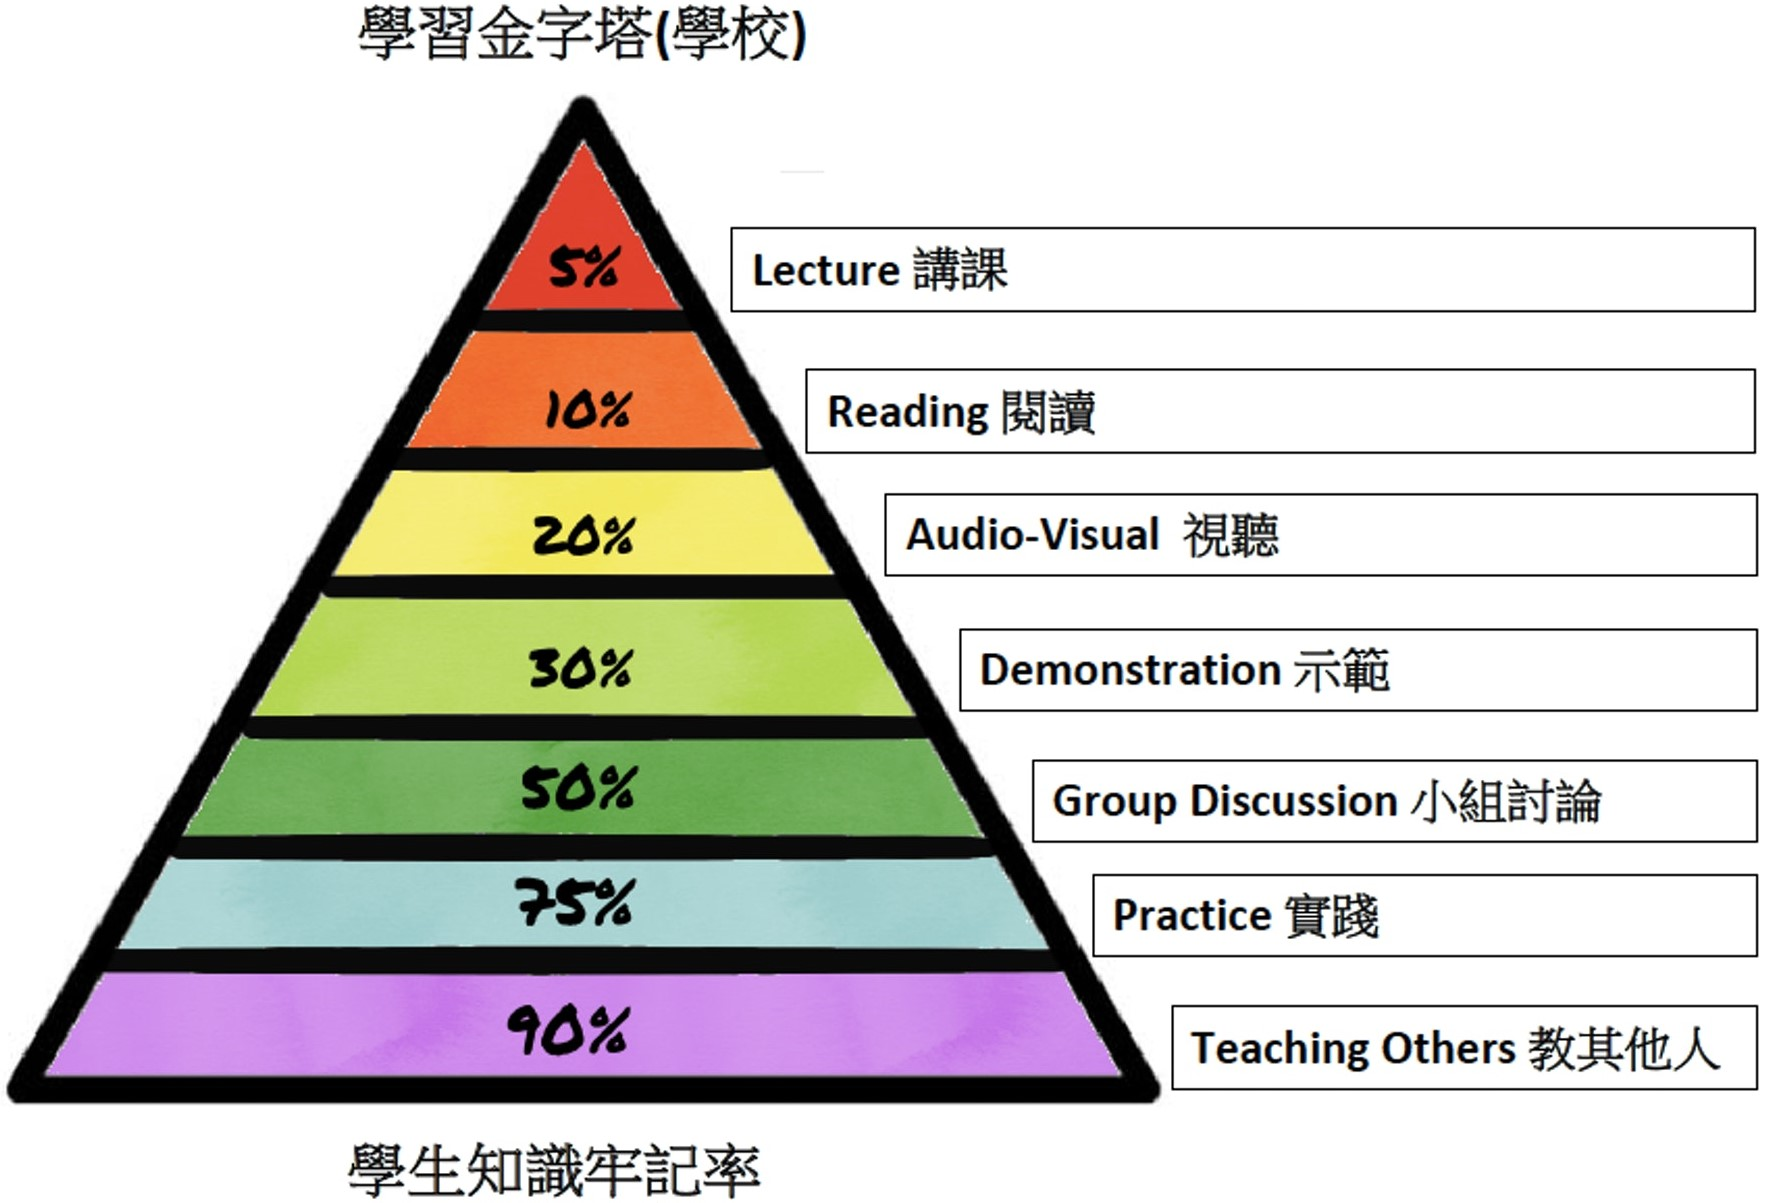
\includegraphics[width=4in]{21}
\caption{\large 學習金字塔}\label{fig.學習金字塔}
\end{center}
\end{figure}
\par

\renewcommand{\baselinestretch}{20} %設定行距
\section{數位化學習環境}
\par
\renewcommand{\baselinestretch}{1} %設定行距
\twelve 於是在數位化的社會下,開始有許多人利用網際內容資源,提供一個數位化學習環境,提升教學品質。\\
\par
\renewcommand{\baselinestretch}{1} %設定行距
\twelve 相比於一般學校裡的教學環境,數位化的網路教學系統可以更容易地設計出讓「使用者主動學習」的教學環境,比如架立討論平台,建立個人專案紀錄歷程檔案......。
\par

\renewcommand{\baselinestretch}{20} %設定行距
\subsection{如何設計出教學環境}
\par
\renewcommand{\baselinestretch}{1} %設定行距
\twelve 首先,我們可以透過費曼學習法,區分主動與被動學習,並分析出教學中,適合引導使用者行主動學習的要素,如以下的方式。
\begin{enumerate}
	\item 課程目標
	\begin{itemize}
		\item 為什麼要開這門課?
		\item 開這門課的目的是什麼?
		\item 希望達成什麼樣的目標?
		\item 希望解決什麼樣的問題?
		\item 達成這樣的目標對於個人、社會、世界會發生什麼樣的影響?
	\end{itemize}
	\item 理論基礎
	\begin{itemize}
		\item 為達成前述的目標,應該要如何結構一門課?
		\item 什麼樣的理論基礎及知識觀點可以支撐起這個架構?
	\end{itemize}
	\item 教學題材
	\begin{itemize}
		\item 選用什麼題材可以反應真實世界概況?
		\item 什麼實例可以串接學生及生活世界之間的距離?
		\item 什麼內容可以與時俱進並體現時代的脈動?
	\end{itemize}
「教學」中值得「研究」的元素
	\item 教學方法
	\begin{itemize}
		\item 設計何種教法可以合適地表達教材的意義?
		\item 規劃什麼樣的活動可以激發學生的動機,並且深化學習的意義?
	\end{itemize}
	\item 學生學習
	\begin{itemize}
		\item 學生如何建構對於知識的理解?
		\item 如何形成相關的態度?
		\item 學生學習及認知的過程為何?
	\end{itemize}
	\item 成果評量
	\begin{itemize}
		\item 經過教學之後,整體課程的效果如何?
		\item 如何明確地評量?
	\end{itemize}
\end{enumerate}
\par

\renewcommand{\baselinestretch}{20} %設定行距
\section{數位教育資源的實體功能}
\par
\renewcommand{\baselinestretch}{1} %設定行距
\twelve 分析完教學中,適合引導使用者主動學習的要素後,針對上述要點,我們可以規劃出一系列的教學網站結構。
\begin{enumerate}
	\item 測驗練習: 用軟體做題,不用等待老師長時間的批改,自己馬上就能知道自己的薄弱環節。
	\item 測驗詳解: 測驗完,針對自己不太會的,可以看到答題詳解,立即更正原本錯誤的觀念。
	\item 互動平台: 傳統的課堂,由於時間有限,無法廣泛聽取所有同學的觀點,再加上青春期的特點,即使有想法,有些孩子也總是羞於舉手回答,一定程度上影響了表達和共享,老師也很難知道學生的情況。課堂交流也不一定要面對面,讓學習跨越時空,一對一的課堂問答模式變成了面向全體的在線問答。多對多課堂模式,所有學生都可以看到「班級問答」區的問題,如此,交流不再是少部分同學的特權,每個人的機會都是均等的,這也在某種程度上重塑學生學習的信心。在線問答和交流,所有孩子都有機會及時整理自己的知識和想法,老師也能真正和孩子們互動起來。這種模式下的學習,打破了課堂時間和空間位置的束縛,增大信息流量,實現全班同學的思維互動。同時,也發揮了部分學有餘力的同學的資源優勢,最終提高了全體學生的學習積極性和學習績效。
	\item 個人紀錄: 查看已發觀點並進行適當地調整,最終將自己的觀點整理輸出。
	\item 背景後台: 針對不同的使用者,開放不同的權限,老師可以上傳了海量的學習資源,一鍵將不同難度的視頻推送給不同層次的學生;利用它進行課堂學習,同時也能給程度不一致的學生設置不同的課後習題,並且觀察到後台大數據,瞬間分析出每一個學生的作業正確率和做題速度等,每個學生解題答案老師一清二楚。
\end{enumerate}
\par
\renewcommand{\baselinestretch}{1} %設定行距
\twelve 將教師從知識的搬運工變成課堂教學活動的設計者、組織者、指導者與參與者;把學生從知識的背誦者、接受者變為知識的實踐者、探索者和創造者,自動學習,學會分享交流,並在討論中觸發創新,實現自主化、個性化的學習。
\par

\renewcommand{\baselinestretch}{20} %設定行距
\section{網際網路-遠距新趨勢}
\par
\renewcommand{\baselinestretch}{1} %設定行距
\twelve
\begin{enumerate}
	\item 電子郵件: 學生可利用電子郵件接收課程教材、作業分配、班級的相關資訊、並與教師、同學或不同年紀的學生相互溝通。教師也可另外設定一個課程討論群組(course listserv),所有的討論和問題都會寄到課程討論群組的電子郵件寄住信箱來,系統會自動將這些内容再寄給各組成員。
	\item 公告欄: 學生直接將自己的討論和間題張貼(post)在公告欄、公開討論區或新閒群組上,以相互溝通。使用者必須連到主機伺服器去閱覽這些文章。這樣可以有組纖的交談,因爲使用者可以選擇自己有興趣的主題進行閱讀和回應。
	\item 資料下載
學生可透過以下幾種方式獲取教學資料:利用檔案傳輸下載文件、教材或軟體;公告欄下載主題文章:全球資訊網下載所需的資料。這些資料下載之後:可在學生的電腦中閱讀或列印。這種方式最缺乏互動性,但卻是透過網際網路進行遠距教學或训練最常使用的方式。
	\item 互動式個別指導教材(Interaotive tutorial)
學生連線到網際網路上(通常是全球資訊網,並在線上取得個別指導教材。道些教材包括閱讀資料、連結到新的網站、回答問題或測驗等。有些個別指導教材允許學生依照自己的速度進行學習,每次連線進來都可繼續上次未完成的學習。
	\item 即時互動會議系統(Real-time Conference)
電子佈告欄和電子郵件在遠距學習的環境中屬於非同步學習。而「即時互動會議系統」則屬於同步學習,教師與學生同時在線上進行面對面的教學與討論。這是最接近傅統教室教學情境的一種方式,教師與學生或學生之間可即時的交談與間答。即時互動會議系統可採用多物件導向系統(Muti-user Object Oriented; MOOs),這是一個可以讓許多使用者同時進入的互動系統,例如網路聊天室 (Internet Relay Chat ; IRC) 便提供了許多即時學習和互動的機會。
	\item 全球資訊網: 以多媒體的方式(如文字、圖片。影像、動畫、聲音,等)提供各式各樣的資訊。大部份全球賌訊網的瀏覽器可以同時使用檔案找尋系統(Archie)、檔案傳輸、資料查詢服務系統、新閒論壇、電子郵件等資源。教師與學生可利用上述資源搜尋、列印、和下載資訊。全球資訊網不僅能夠整合網路的資源,還可讓使用者以建立網頁(Homepage)的方式,來成爲個人資訊提供者,而不單只是一個資訊使用者。道種整合運用資訊及讓使用者參與資訊建設的功能,使全球資訊網成為不可忽融的新教學媒體。
\end{enumerate}
\par














%=------------------提升研究效益----------------------=%
%\newpage
%\chapter{網際內容如何提升研究效益}
\renewcommand{\baselinestretch}{10} %設定行距
%\section{前言}
\par
\renewcommand{\baselinestretch}{1} %設定行距
\twelve
\par

%=------------------分散式系統----------------------=%
%\newpage
%\chapter{分散式系統}
\renewcommand{\baselinestretch}{10} %設定行距
\section{前言}
\par
\renewcommand{\baselinestretch}{1} %設定行距
\twelve \qquad 要合作就必須溝通與協調,俗話說合作就是力量大,但是溝通與協調不僅僅是一種本能,更是一種能力。這就是分散式運算的問題來源,在分散式環境中,合作對象是分散各地的電腦,在這些電腦透過網路連接在一起,每台電腦都能讀立運行,且同時也能藉由分散式系統來進行合作,若以一個基層人員而言,需要將上級、同級、下級,甚至客戶,的每一件事項在對應的部分做串聯,甚至獨立解決,而產生一加一大於二的成效。
\par
\renewcommand{\baselinestretch}{20} %設定行距
\section{分散式系統的基本架構}
\par
\renewcommand{\baselinestretch}{1} %設定行距
\twelve \qquad 
\par
\renewcommand{\baselinestretch}{20} %設定行距

\section{事件的排序問題}
\par
\renewcommand{\baselinestretch}{1} %設定行距
\twelve \qquad 
\par}

%=------------------伺服器架構----------------------=%
%\newpage
%\chapter{伺服器架構}
\renewcommand{\baselinestretch}{10} %設定行距
%\section{前言}
\par
\renewcommand{\baselinestretch}{1} %設定行距
\twelve \qquad 此專題採用Windows 10版本作為我們的架設所使用作業系統,Windows作業系統在作業系統中的市佔率高達七成五以上,且Windows 10作業系統在Windows作業系統中的使用率高達八成以上。
\\
\par
\renewcommand{\baselinestretch}{1} %設定行距
\twelve \hspace{0.5em} 以下為Windows作業系統與Linux作業系統的比較。
\par
\\
\begin{center}
\begin{tabular}{|l|p{6.5cm}|p{6.5cm}|} %表格
\hline
比較&Windows&Linux 
\\
\hline
介面&介面統一,所有Windows程式選單幾乎一致。&圖形介面風格依發行版不同而不同,可能互不相容。
\\
\hline
使用&使用比較簡單,容易入門。圖形化介面對沒有電腦背景知識的使用者使用十分有利&命令列介面,需要學習才能掌握,但也有圖形介面使用上,也較令另列易上手。
\\
\hline
學習&系統構造複雜、變化頻繁,且知識、技能淘汰快,深入學習困難。&系統構造簡單、穩定,且知識、技能傳承性好,深入學習相對容易。
\\
\hline
軟體&商業軟體為主。有很多軟體只能在windows裏運行,無法相容Linux。&自由軟體為主。Linux相容的軟體有需多處於開發中,選擇性相對Windows較少。
\\
\hline
使用者&七成五以上。&不到一成。
\\
\hline
\end{tabular}
\end{center}
\par

\renewcommand{\baselinestretch}{20} %設定行距
\section{Windows 環境配置}
\par
\renewcommand{\baselinestretch}{1} %設定行距
\twelve \qquad 在Window系統安裝完成後,將所需要的軟體安裝到系統上,之後將安裝的軟體在系統上設定環境變數。
\\
\par
\renewcommand{\baselinestretch}{1} %設定行距
\twelve \hspace{0.5em} 環境變數是一個動態命名的值,可以影響電腦上行程的行為方式,使用者通過設定環境變數,來更好的執行程序。
\\
\par
\renewcommand{\baselinestretch}{1} %設定行距
\twelve \hspace{0.5em} 在作業系統搜尋如(圖\ref{fig.關鍵字})
\\
\par
\renewcommand{\baselinestretch}{1.7} %設定行距
\begin{figure}[hbt!]
\begin{center}

\includegraphics[width=3in]{5}
\caption{\large 關鍵字}\label{fig.關鍵字}
\end{center}
\end{figure}
\par
\\
\renewcommand{\baselinestretch}{1} %設定行距
\twelve \hspace{0.5em} 選擇環境變數如(圖\ref{fig.環境變數})
\\
\par
\renewcommand{\baselinestretch}{1.7} %設定行距
\begin{figure}[hbt!]
\begin{center}
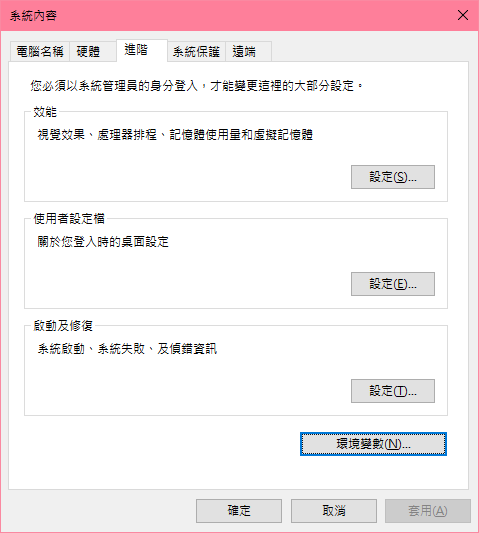
\includegraphics[width=5in]{6}
\caption{\large 環境變數}\label{fig.環境變數}
\end{center}
\end{figure}
\par
\\
\renewcommand{\baselinestretch}{1} %設定行距
\twelve \hspace{0.5em} 選擇系統變數中的Path如(圖\ref{fig.Path})
\\
\par
\renewcommand{\baselinestretch}{1.7} %設定行距
\begin{figure}[hbt!]
\begin{center}
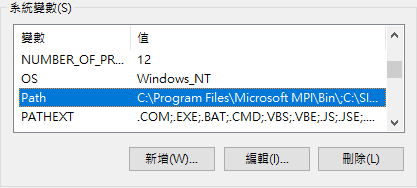
\includegraphics[width=4in]{7}
\caption{\large Path}\label{fig.Path}
\end{center}
\end{figure}
\par
\\
\renewcommand{\baselinestretch}{1} %設定行距
\twelve \hspace{0.5em} 新增變數並且指定路徑如(圖\ref{fig.編輯環境變數})
\\
\par
\renewcommand{\baselinestretch}{1.7} %設定行距
\begin{figure}[hbt!]
\begin{center}
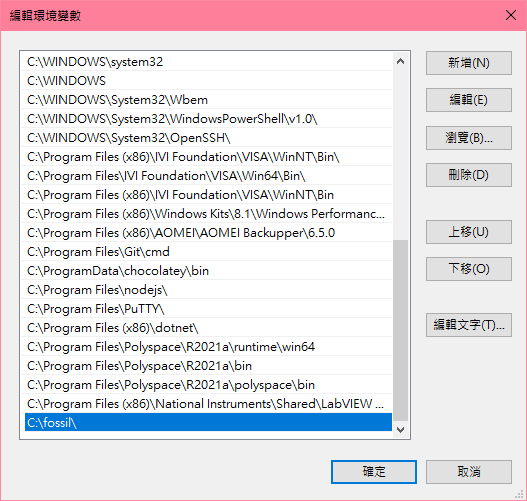
\includegraphics[width=5in]{8}
\caption{\large 編輯環境變數}\label{fig.編輯環境變數}
\end{center}
\end{figure}
\par

\renewcommand{\baselinestretch}{20} %設定行距
\section{Fossil SCM}
\par
\renewcommand{\baselinestretch}{1} %設定行距
\twelve \qquad 對於研究或專案計畫而言,工作中經常使用的具是電腦或其他相關電子產品,而對於研究過程或開發的流程、錯誤及解果的每個步驟都相刀的重要,而對負責軟體開發工作的軟體團隊成員來說,版本控制系統是一套相當重要的軟體工具。如果沒有版本控制系統,開發團隊成員將難以有效控制研究或開發過程,並可能導致效率的增加。
\\
\par
\renewcommand{\baselinestretch}{1} %設定行距
\twelve \hspace{0.5em} 目前已經存在許多成熟的版本控制系統,例如較為知名的 Git、Subversion或CVS等等。若以架設方式加以細分,則有分散式與Client-Server二種不同的系統分類。除了這些系統以外,網路上還可以找到許多其他各具特色的版本控制系統。雖然這些系統的知名度較低,但如果仔細檢視其優點與特色,仍然可以找到一些頗為出色的版本控制系統。
\\
\par
\renewcommand{\baselinestretch}{1} %設定行距
\twelve \hspace{0.5em} 因此本專題所使用的是Fossil,是一套採用分散式處理方式的版本控制系統。
\\
\par
\renewcommand{\baselinestretch}{1.7} %設定行距
\begin{figure}[hbt!]
\begin{center}

\includegraphics[width=1in]{9}
\caption{\large Fossil}\label{fig.Fossil}
\end{center}
\end{figure}
\par
\\
\renewcommand{\baselinestretch}{1} %設定行距
\twelve \hspace{0.5em} 因此本專題所使用的是Fossil,是一套採用分散式處理方式的版本控制系統。
\par

\renewcommand{\baselinestretch}{20} %設定行距
\subsection{特色}
\par
\renewcommand{\baselinestretch}{1} %設定行距
\twelve \qquad 一般人對於軟體本身的使用需求,多半是希望越容易操作越好,並且有相當程度的穩定性與可靠性。而操作簡單與系統本身穩定性高,正是Fossil所強調的二大重點。
\\
\par
\renewcommand{\baselinestretch}{1} %設定行距
\twelve \hspace{0.5em} 在穩定性方面,Fossil採用SQLite資料庫作為儲存的平台,再加上永久性的檔案結構,即使遭遇斷電或是元件(不包括硬碟)損毀等問題,資料也不會損失。
\\
\par
\renewcommand{\baselinestretch}{1} %設定行距
\twelve \hspace{0.5em} 在可靠性方面,Fossil目前也正在研發新的保護機制,在未來的版本中將會提供自動檢查機制,只要資料提交,系統便會自動進行資料內容驗證,以確保資料內容無誤,以提升可靠性。
\\
\par
\\
\renewcommand{\baselinestretch}{1} %設定行距
\twelve \hspace{0.5em} Fossil之所以可以作為官方網站的平台,是因為除了版本控制系統相關的功能以外,亦可利用Fossil作為Blog 平台的架設方案。所以無論使用者需要的是單純的版本控制,或是希望架設網站作為資訊分享的平台,都能利用Fossil一併解決。所以在取得Fossil之後,不只獲得Fossil本身的原始碼,還取得了一整個網站系統的架設方案。
\par
\\

\renewcommand{\baselinestretch}{20} %設定行距
\subsection{功能}
\par
\renewcommand{\baselinestretch}{1} %設定行距
\begin{enumerate}
	\item \textbf{項目管理:} 除了像Git和Mercurial那樣做分佈式版本控制之外,Fossil還支持錯誤追蹤、wiki、論壇、電子郵件警報、聊天和技術說明。
	\item \textbf{Web介面:} Fossil具有內置、主題化、可擴展和直觀的Web界面,其中包含豐富多樣的信息頁面。
	\item \textbf{一體式:} Fossil是一個獨立的、獨立的可執行文件。要安裝,只需下載適用於Linux、Mac或Windows的預編譯二進製文件,並將其放在PATH上。還提供易於編譯的源代碼。
	\item \textbf{自託管:} 使用各種技術在幾分鐘內建立一個項目網站。Fossil具有CPU和內存效率。大多數項目可以舒適地託管在每月5美元的VPS 或Raspberry Pi上。還可以設置自動GitHub鏡像。
	\item \textbf{簡單網路系統:} Fossil使用普通的Https或Ssh進行網絡通信,因此它可以在防火牆和代理後面正常工作。該協議帶寬效率很高,以至於Fossil可以通過撥號、弱3G或客機Wifi輕鬆使用。
	\item \textbf{自動同步:} Fossil支持自動同步模式,通過減少與分佈式項目相​​關的不必要的分叉和合併數量,有助於保持項目向前發展。
	\item \textbf{開源:} BSD授權條款。
\end{enumerate}
\par

\renewcommand{\baselinestretch}{20} %設定行距
\subsection{Fossil 操作簡介}
\par
\renewcommand{\baselinestretch}{1} %設定行距
\twelve \qquad Fossil與其他版本控制系統相同,主要使用的都是儲存庫(Repository)的概念。儲存庫可以視為一種資料庫,其中存放了專案相關的檔案與資料等等。使用者處理這些檔案時,需要先將資料取出(Check Out)並存放至本地端中,也就是使用者的工作目錄。等到完成了新增、修改等各種工作,再將本地端的資料回存(Check In)至儲存庫之中,即可完成整個處理作業。也就是說,在使用Fossil時,主要的動作有三項:新增或複製儲藏庫、取出資料、進行資料處理與存取等工作。
\\
\par
\renewcommand{\baselinestretch}{1} %設定行距
\twelve \hspace{0.5em} 專ㄋ案開始執行時,需要新增一個儲藏庫,此時可以使用下列指令,建立一個新的儲存庫。儲存庫名稱未限制,因此可以使用任何命名方式,也可以不用使用任何副檔名。
\par
\begin{center}
\begin{tabular}{||p{15cm}|} %表格
\hline
\textbf{fossil init} \emph{repository-filename}
\\
\hline
\end{tabular}
\end{center}
\par
\renewcommand{\baselinestretch}{1} %設定行距
\twelve \hspace{0.5em} 儲存庫是以檔案方式存在於系統之中,所以執行此指令之後,便可在檔案系統中找到以儲存庫名稱命名的檔案。大多數Fossil的操作都針對本地的儲存庫進行處理,如果需要存取遠端系統中的儲存庫,以下列指令將遠端儲存庫複製到本地中,再進行後續處理。
\par
\begin{center}
\begin{tabular}{||p{15cm}|} %表格
\hline
\textbf{fossil clone} \emph{https://your-id-num@your-domain-name/ your-db.fossil}
\\
\hline
\end{tabular}
\end{center}
\par
\renewcommand{\baselinestretch}{1} %設定行距
\twelve \hspace{0.5em} 建立或複製完儲存庫之後,此時可以先建立一個新目錄,切換到此目錄並且以下列指令展開取得\_ FOSSIL\_ 檔案。
\par
\begin{center}
\begin{tabular}{||p{15cm}|} %表格
\hline
\textbf{fossil open} \emph{repository-filename}
\\
\hline
\end{tabular}
\end{center}
\par
\renewcommand{\baselinestretch}{1} %設定行距
\twelve \hspace{0.5em} 此時可以將所需提交的檔案放置此目錄,並且以下列指令將指定的檔案加入到儲存庫。
\par
\begin{center}
\begin{tabular}{||p{15cm}|} %表格
\hline
\textbf{fossil add} \emph{file...}
\\
\hline
\end{tabular}
\end{center}
\par
\renewcommand{\baselinestretch}{1} %設定行距
\twelve \hspace{0.5em} 若需要儲存庫的資料刪除,以下列指令將指定的檔案刪除於儲存庫。
\par
\begin{center}
\begin{tabular}{||p{15cm}|} %表格
\hline
\textbf{fossil rm} \emph{file...}
\\
\hline
\end{tabular}
\end{center}
\par
\renewcommand{\baselinestretch}{1} %設定行距
\twelve \hspace{0.5em} 如果覺得依序加入或移除檔案的方式有些麻煩,則可以以下列指令,讓儲存庫與本地目錄中的檔案清單自動的做對比,如果有檔案存在於本地目錄,但並未在儲存庫之中出現,則會自動將此檔案加入儲存庫之中。相反的,如果檔案只出現在儲存庫,但本地目錄中找不到該檔案,則會自動將此檔案自儲存庫之中移除。
\par
\begin{center}
\begin{tabular}{||p{15cm}|} %表格
\hline
\textbf{fossil addremove}
\\
\hline
\end{tabular}
\end{center}
\par
\renewcommand{\baselinestretch}{1} %設定行距
\twelve \hspace{0.5em} 當新增或刪除的部分完成時,需要以下列指令做最後的提交,所新增或刪除的檔案才會正式生效。
\par
\begin{center}
\begin{tabular}{||p{15cm}|} %表格
\hline
\textbf{fossil commit}
\\
\hline
\end{tabular}
\end{center}
\par
\renewcommand{\baselinestretch}{1} %設定行距
\twelve \hspace{0.5em} 以上僅是Fossil最基本的操作方式,並未完整涵蓋Fossil所有的指令與其參數。以下為Fossil經常使用的指令。
\\
\par
\begin{center}
\begin{tabular}{|p{2cm}|p{2cm}|p{2cm}|p{2cm}|p{2cm}|p{2cm}|} %表格
\hline
add          &cat          &diff         &ls           &remote       &tag
\\
\hline
addremove    &changes      &extras       &merge        &revert       &timeline
\\
\hline
all          &chat         &finfo        &mv           &rm           &ui
\\
\hline
amend        &clean        &gdiff        &open         &settings     &undo
\\
\hline
annotate     &clone        &grep         &patch        &sql          &unversioned
\\
\hline
bisect       &commit       &help         &pull         &stash        &update
\\
\hline
blame        &dbstat       &info         &push         &status       &version
\\
\hline
branch       &delete       &init         &rebuild      &sync         &xdiff
\\
\hline
\end{tabular}
\end{center}

\clearpage %換頁
\renewcommand{\baselinestretch}{20} %設定行距
\section{Stunnel}
\par
\renewcommand{\baselinestretch}{1} %設定行距
\twelve \qquad Stunnel是一種代理,旨在將TLS加密功能添加到現有客戶端和服務器,而無需對程序代碼進行任何更改。 它的架構針對安全性、可移植性和可擴展性(包括負載平衡)進行了優化,使其適用於大型部署。
\\
\par
\renewcommand{\baselinestretch}{1.7} %設定行距
\begin{figure}[hbt!]
\begin{center}

\includegraphics[width=2.5in]{12}
\caption{\large Stunnel}\label{fig.Stunnel}
\end{center}
\end{figure}
\par

\subsection{功能}
\renewcommand{\baselinestretch}{1} %設定行距
\begin{itemize}
	\item 可移植性(線程模型)
	\item 性能和可擴展性
	\item 支持 OpenSSL 安全功能
	\item 其他跨平台功能
	\item Unix 特性
	\item Windows功能	
\end{itemize}
\par

\renewcommand{\baselinestretch}{20} %設定行距
\subsection{為何要使用Stunnel?}
\par
\renewcommand{\baselinestretch}{1} %設定行距
\twelve \qquad 資料在網路傳輸下,如(圖\ref{fig.普通網路})若沒有經過任何保護等機制,當網路遭受駭客或其他網路攻擊時,容易造成資料被竊取,因此為了使網路在傳輸下是安全的,因此使用Stunnel。
\\
\par
\renewcommand{\baselinestretch}{1.7} %設定行距
\begin{figure}[hbt!]
\begin{center}
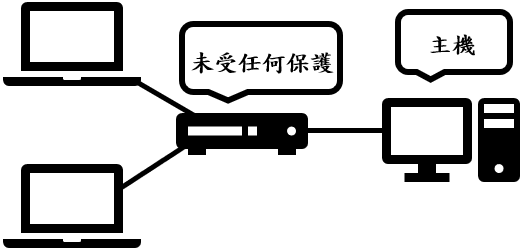
\includegraphics[width=3in]{10}
\caption{\large 普通網路}\label{fig.普通網路}
\end{center}
\end{figure}
\par

\newpage

\renewcommand{\baselinestretch}{1} %設定行距
\twelve \hspace{0.5em} Stunnel是一個可以用SSL對任意TCP連接加密的程式,並可工作在Unix和Windows平臺上。它採用Client/Server模式,將Client端的網路資料採用SSL加密後,安全的傳輸到指定的Server端再進行解密還原,然後再發送到訪問的伺服器。在加密傳輸過程中,可充分確保資料的安全性,我們只要把Server端程式安裝在局域網外的一台伺服器上,即可保證傳輸的資料在局域網內是安全的,如(圖\ref{fig.加密網路})。
\\
\par
\renewcommand{\baselinestretch}{1.7} %設定行距
\begin{figure}[hbt!]
\begin{center}
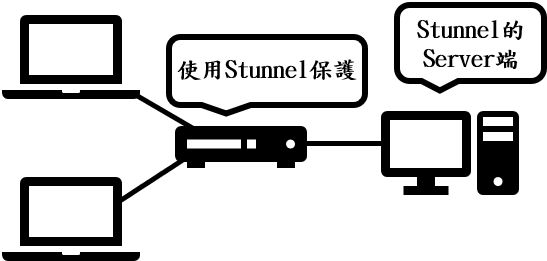
\includegraphics[width=3in]{11}
\caption{\large 加密網路}\label{fig.加密網路}
\end{center}
\end{figure}
\par

\renewcommand{\baselinestretch}{20} %設定行距
\subsection{設定操作}
\par
\renewcommand{\baselinestretch}{1} %設定行距
\twelve \qquad 因為要將Fossil採用Https內容與Stunnel互動。因此與Stunnel Https結合,此外需要將stunnel.conf設定如下。
\\
\par
\begin{center}
\begin{tabular}{||p{15cm}|} %表格
\hline
[https]
\\
accept = pj5073.cycu.org:443
\\
connect = 9000
\\
cert = fullchain.pem
\\
key = privkey.pem
\\
TIMEOUTclose = 0
\\
\hline
\end{tabular}
\end{center}
\par
\renewcommand{\baselinestretch}{1} %設定行距
\twelve \hspace{0.5em} 原本使用的cert與key是使用localhost.crt與localhost.key為自簽章憑證,自簽章憑證一樣可以用來加密,但是由於該憑證不屬於公開金鑰基礎建設簽發憑證,其他沒信任該憑證的Https存取者的網頁瀏覽器會顯示一個警告,說這個憑證不被他們的電腦或瀏覽器信任。因此必須接受數位簽章的public key,因此cert與key目前已經設定為public key,此部分由後續的3.6 Let's Encrypt章節所探討。
\par

\renewcommand{\baselinestretch}{20} %設定行距
\subsection{負載平衡}
\par
\renewcommand{\baselinestretch}{1} %設定行距
\twelve \qquad 用來在多個電腦、網路連接、CPU、磁碟驅動器或其他資源中分配負載,以達到最佳化資源使用、最大化吞吐率、最小化回應時間、同時避免過載的目的。使用帶有負載平衡的多個伺服器組件,取代單一的組件,可以通過冗餘提高可靠性。
\\
\par
\renewcommand{\baselinestretch}{1} %設定行距
\twelve \hspace{0.5em} 利用Stunnel將本地服務器的IP地址與端口port 9000、5000、5001、9001的資訊,分別轉給外部的客戶端連接端口443、8443、9443、5443的Https協定連線,設定如下。

\par
\begin{center}
\begin{tabular}{||p{15cm}|} %表格
\hline
[https]
\\
accept  = pj5073.cycu.org:443
\\
connect = 9000
\\
cert = fullchain.pem
\\
key = privkey.pem
\\
TIMEOUTclose = 0
\\
\\ 
[https]
\\
accept = pj5073.cycu.org:8443
\\
connect = 5000
\\
cert = fullchain.pem
\\
key = privkey.pem
\\
TIMEOUTclose = 0
\\
\\
[https]
\\
accept = pj5073.cycu.org:9443
\\
connect = 5001
\\
cert = fullchain.pem
\\
key = privkey.pem
\\
TIMEOUTclose = 0
\\
\\
[https]
\\
accept = pj5073.cycu.org:5443
\\
connect = 9001
\\
cert = fullchain.pem
\\
key = privkey.pem
\\
TIMEOUTclose = 0
\\
\hline
\end{tabular}
\end{center}
\par

\renewcommand{\baselinestretch}{20} %設定行距
\section{Nginx}
\par
\renewcommand{\baselinestretch}{1} %設定行距
\twelve \qquad Nginx是一個免費的開源軟體,一個非同步框架的web server,不過它的功用遠不僅止於web server,它更多的用途是作為反向代理、Http服務、負載平衡器甚至還可以處理靜態資源、代理等等工作。
\\
\par
\renewcommand{\baselinestretch}{1.7} %設定行距
\begin{figure}[hbt!]
\begin{center}

\includegraphics[width=3in]{13}
\caption{\large Nginx}\label{fig.Nginx}
\end{center}
\end{figure}
\par

\renewcommand{\baselinestretch}{20} %設定行距
\subsection{設定操作}
\par
\renewcommand{\baselinestretch}{1} %設定行距
\twelve \qquad 其中安裝Nginx全球資訊網伺服器的目的之一,為後續使用Certbot套件,能夠取得www伺服器透過直接驗證網站的符號名稱,因此取得公證數位簽章的第一步是安裝Nginx,此部分由後續的3.6 Let's Encrypt章節所探討,而安裝Nginx的另外一個用處是,可以利用Html Redirect的方式,將Http連線跳轉到Https設定如下。
\\
\begin{center}
\begin{tabular}{||p{15cm}|} %表格
\hline
server \{
\\
\qquad listen \qquad \qquad [::]:80 default ipv6only=on;
\\
\qquad server\_ name \quad pj5073.cycu.org;
\\
\}
\\
\hline
\end{tabular}
\end{center}
\par
\renewcommand{\baselinestretch}{1} %設定行距
\twelve \hspace{0.5em} 由於pj2022.cycu.org目前只開放IPv6網域,因此在設定Nginx的時候,必須注意是否啟動listen IPv6 網路協定封包。
\par
\renewcommand{\baselinestretch}{1} %設定行距
\twelve \hspace{0.5em} 設定如下為接受IPv6封包。
\par
\begin{center}
\begin{tabular}{||p{15cm}|} %表格
\hline
listen [::]:80
\\
\hline
\end{tabular}
\end{center}
\par
\renewcommand{\baselinestretch}{1} %設定行距
\twelve \hspace{0.5em} 設定如下為接受IPv4封包。另外就是server\_name 設定為所指定網域,應該就可以啟動Nginx。
\par
\begin{center}
\begin{tabular}{||p{15cm}|} %表格
\hline
listen :80
\\
\hline
\end{tabular}
\end{center}
\par

\renewcommand{\baselinestretch}{20} %設定行距
\subsection{負載平衡}
\par
\renewcommand{\baselinestretch}{1} %設定行距
\twelve \qquad Nginx提供以下三種負載平衡的方法。
\begin{enumerate}
	\item round-robin:預設值,會將請留輪流平均分配到每台伺服器上。
	\item lest-connected:會將請求分配到目前連接數最少的伺服器上。
	\item ip-hash:利用hash-function來決定使用者要被分配到的伺服器,此方法可以達到同一個使用者(IP address)每次連結的伺服器都是相同的。
\\
\end{enumerate}
\par
\renewcommand{\baselinestretch}{1} %設定行距
\twelve \hspace{0.5em} 設定如下,如果要默認值改成上述的任何一個方法,只需要在round-robin;的行列,將參數改為lest-connected;或ip-hash;即可成為相對應功能。
\par
\begin{center}
\begin{tabular}{||p{15cm}|} %表格
\hline
upstream myweb \{
\\
\qquad round-robin;
\\
\qquad server doamin1.com;
\\
\qquad server domain2.com;
\\
\qquad server domain3.com;
\\
\}
\\
server \{
\\
\qquad listen 80;
\\
\qquad location / \{
\\
\qquad \quad proxy\_ pass \quad http://backend;
\\
\quad \}
\\
\}
\\
\hline
\end{tabular}
\end{center}
\par

\renewcommand{\baselinestretch}{20} %設定行距
\subsection{分配權重 weight}
\par
\renewcommand{\baselinestretch}{1} %設定行距
\twelve \qquad weight默認值為1,設定如下的配置代表如果有5次新的請求,則會有3次被分配到domain1和分配各1次到domian2、domain3的服務區域。
\par
\begin{center}
\begin{tabular}{||p{15cm}|} %表格
\hline
upstream myweb \{
\\
\qquad round-robin;
\\
\qquad server doamin1.com; \quad weight=3;
\\
\qquad server domain2.com;
\\
\qquad server domain3.com;
\\
\}
\\
server \{
\\
\qquad listen 80;
\\
\qquad location / \{
\\
\qquad \quad proxy\_ pass \quad http://backend;
\\
\quad \}
\\
\}
\\
\hline
\end{tabular}
\end{center}
\par

\renewcommand{\baselinestretch}{20} %設定行距
\subsection{備份 backup}
\par
\renewcommand{\baselinestretch}{1} %設定行距
\twelve \qquad 設定如下將部分server作為備份,平時正常使用的時候備用server不生效,當所有伺服器都掛掉之後,此伺服器才會生效,作為異常備份機制。
\par
\begin{center}
\begin{tabular}{||p{15cm}|} %表格
\hline
upstream myweb \{
\\
\qquad round-robin;
\\
\qquad server doamin1.com; \quad weight=3;
\\
\qquad server domain2.com;
\\
\qquad server domain3.com;
\\
\}
\\
server \{
\\
\qquad listen 80;
\\
\qquad location / \{
\\
\qquad \quad proxy\_ pass \quad http://backend;
\\
\quad \}
\\
\}
\\
\hline
\end{tabular}
\end{center}
\par

\renewcommand{\baselinestretch}{20} %設定行距
\section{Nssm}
\par
\renewcommand{\baselinestretch}{1} %設定行距
\twelve \qquad Nssm是由Non-Sucking Service Manager組成而來,Nssm的功能與srvany非常相似。當系統服務管理器啟動時,它會在註冊表中查找關鍵參數並嘗試啟動Application中列出的程序,從AppDirectory中列出的目錄開始,並傳遞列出的選項標誌在AppParameters中。這些值與srvany讀取的值相同,這意味著可以將Nssm用作直接替換,可以把一般Windows程式設定成服務狀態來執行與管理。
\\
\par}
\renewcommand{\baselinestretch}{1.7} %設定行距
\begin{figure}[hbt!]
\begin{center}

\includegraphics[width=1.5in]{14}
\caption{\large Nssm}\label{fig.Nssm}
\end{center}
\end{figure}
\par

\renewcommand{\baselinestretch}{20} %設定行距
\subsection{操作設定}
\par
\renewcommand{\baselinestretch}{1} %設定行距
\twelve \qquad 將nssm.exe安裝於主機,並且將參數設定為環境變數由3.1 Windows環境配置章節說明,接下來設定可分為命令列和圖形介面兩種方式來作為設定,本部分使用圖形介面來做為設定。Fossil、Nginx、Python等等都需要使用Nssm作為服務狀態來執行與管理。
\par
\renewcommand{\baselinestretch}{1} %設定行距
\twelve \hspace{0.5em} 以下列指令,啟用Nssm圖形介面。
\par
\begin{center}
\begin{tabular}{||p{15cm}|} %表格
\hline
\textbf{nssm install} \emph{serviename} 
\\
\hline
\end{tabular}
\end{center}
\par
\renewcommand{\baselinestretch}{1} %設定行距
\twelve \hspace{0.5em} 圖形介面形式如(圖\ref{fig.Nssm GUI})。
\par
\begin{itemize}
	\item Application Path:為參數指定位置。
	\item Startup directory:為參數只指定目錄。
	\item Arguments:參數設定(若無則無須設定)。
	\item Application以外:若無需求則無需設定。
\end{itemize}
\par
\renewcommand{\baselinestretch}{1.7} %設定行距
\begin{figure}[hbt!]
\begin{center}
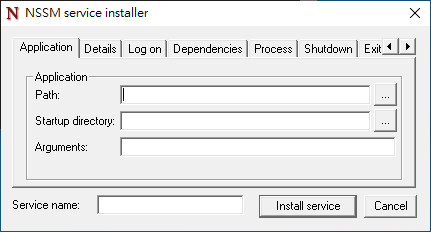
\includegraphics[width=4in]{15}
\caption{\large Nssm GUI}\label{fig.Nssm GUI}
\end{center}
\end{figure}
\par
\renewcommand{\baselinestretch}{1} %設定行距
\twelve \hspace{0.5em} 若設定完成則可以前往工作管理員,確認程序使否成功啟動(圖\ref{fig.程序啟動})。
\par
\renewcommand{\baselinestretch}{1.7} %設定行距
\begin{figure}[hbt!]
\begin{center}
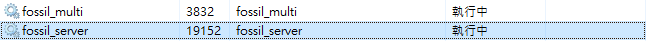
\includegraphics[width=6in]{16}
\caption{\large 程序啟動}\label{fig.程序啟動}
\end{center}
\end{figure}
\par

\renewcommand{\baselinestretch}{20} %設定行距
\section{Let's Encrypt}
\par
\renewcommand{\baselinestretch}{1} %設定行距
\twelve \qquad Let’s Encrypt是一個免費、自動化、開放,為了公眾利益而運作的憑證頒發機構(Certificate Authority,CA)。它是由Internet Security Research Group (ISRG)所提供的服務。為了建立一個更加安全,更尊重隱私的網際網路,免費提供用戶數位憑證,並以最友善的方式替網站啟用Https (SSL/TLS)。
\par
\renewcommand{\baselinestretch}{1.7} %設定行距
\begin{figure}[hbt!]
\begin{center}

\includegraphics[width=3in]{17}
\caption{\large Let's Encrypt}\label{fig.Let's Encrypt}
\end{center}
\end{figure}
\par

\renewcommand{\baselinestretch}{20} %設定行距
\subsection{Certbot}
\par
\renewcommand{\baselinestretch}{1} %設定行距
\twelve \qquad 由於先前於3.3 Stunnel章節所提到數位簽章為自簽憑證,使用者在連線至Https網域則其他使用者是無信任度,因此瀏覽器會顯示一個緊告狀態,此時必須接受數位簽章的public key,瀏覽器才能對使用者信任。因此使用Certbot取得網站符號名稱的正式Https數位簽章。
\\
\par
\renewcommand{\baselinestretch}{1.7} %設定行距
\begin{figure}[hbt!]
\begin{center}

\includegraphics[width=3in]{18}
\caption{\large Certbot}\label{Certbot}
\end{center}
\end{figure}
\par
\renewcommand{\baselinestretch}{1} %設定行距
\twelve \hspace{0.5em} 啟動Nginx且安裝Certbot後,以下列指令執行Certbot。
\par
\begin{center}
\begin{tabular}{||p{15cm}|} %表格
\hline
\textbf{certbot certonly -\ -webroot}
\\
\hline
\end{tabular}
\end{center}
\par
\renewcommand{\baselinestretch}{1} %設定行距
\twelve \hspace{0.5em} 若設定完成,public key則會放置於指定位置,只需將public key放置於stunnel.conf目錄中和將stunnel.conf中的cert和key換成相對應的key,則將程序服務重新啟動即可使用公開數位簽章。
\par

\renewcommand{\baselinestretch}{20} %設定行距
\subsection{Let’s Encrypt的基本原則}
\par
\renewcommand{\baselinestretch}{1} %設定行距
\begin{itemize}
	\item 免費:任何擁有網域名稱的人都可以免費使用Let’s Encrypt取得可信任的憑證。
	\item 自動化:運行於網頁伺服器上的程式可以透過與Let’s Encrypt溝通,輕鬆地獲取憑證,安全地設定並使用它,並且自動進行憑證更新。
	\item 安全:Let’s Encrypt將是推動TLS安全的最佳平台,無論是在CA方面,還是幫助網站營運者正確地保護他們的伺服器。
	\item 透明:公開記錄所有頒發或註銷的憑證,供任何人查閱。
	\item 公開:公開自動頒發和更新協議,作為他人可以使用的開放標準。
	\item 合作:Let’s Encrypt是一個為了網路社群利益所做的共同努力,就像網路底層協議一樣,不受任何單一組織的控制。
\end{itemize}
\par

\renewcommand{\baselinestretch}{20} %設定行距
\subsection{Https流程}
\par
\renewcommand{\baselinestretch}{1} %設定行距
\twelve \qquad 當你提出申請時,Lets' Encrypt就產一個Challenges,你需要讓你的網站可以回傳該資訊,做得到就表示這個網站是你的,接下來就是交換key的動作了。
\\
\par
\begin{figure}[hbt!]
\begin{center}
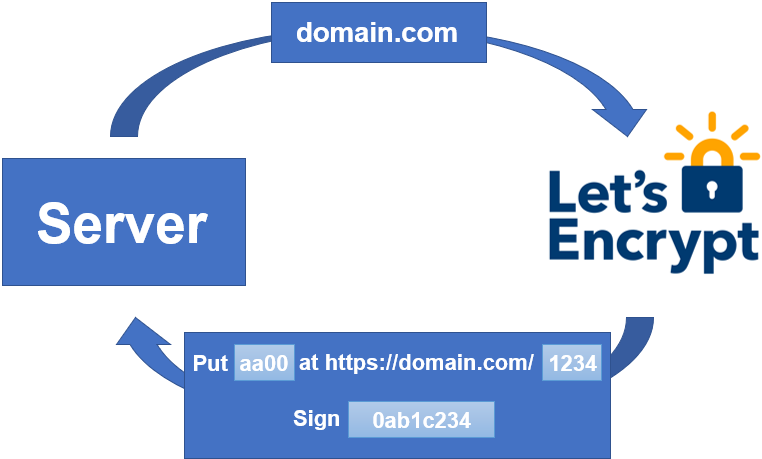
\includegraphics[width=4.5in]{19}
\caption{\large 提交}\label{fig.提交}
\end{center}
\end{figure}
\begin{figure}[hbt!]
\begin{center}
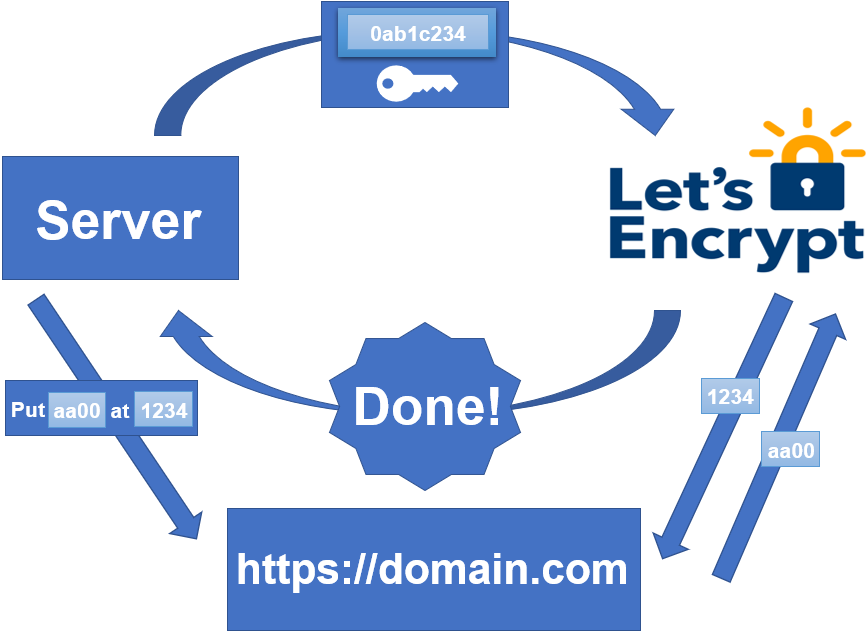
\includegraphics[width=4.5in]{20}
\caption{\large 回應}\label{fig.回應}
\end{center}
\end{figure}
\par

%=------------------Oauth----------------------=%
%\newpage
%\chapter{Oauth}
\renewcommand{\baselinestretch}{10} %設定行距
\par
\renewcommand{\baselinestretch}{1} %設定行距
\twelve OAuth是一個開放標準,張允許用戶讓第三方應用存取該用戶在某一網站上儲存的私密的資源,而無需將用戶名稱和密碼提供給第三方應用,OAuth允許用戶提供一個權杖,而不是用戶名稱和密碼來存取他們存放在特定服務提供者的資料,每一個權杖授權一個特定張的網站在特定的時段內存取特定的資源。\\
\par
\twelve 例如平常在網站上可能需要登入,因此會有Google、Facebook等等選項,選擇某一選項會跳到同意頁面,最後會再轉回來原本的網站,當你點了同意,網站就可以拿到一個token,會到相對應的API取得你剛同意授權的資料。現在有些網站不會有自己的會員系統了,都用這種方式來做登入,好處是資安的問題不用保管使用者的帳密,且也比較省資料空間,對使用者來說也很方便,不用特別申請使用者帳號。

\renewcommand{\baselinestretch}{20} %設定行距
\section{Google Oauth 2.0}
\par
\renewcommand{\baselinestretch}{1} %設定行距
\twelve 因此從Google API Console取得Google OAuth 2.0憑證,接著從Google Authorization Server取得access token,檢查使用者願意提供的資料範圍是否正確,推送access token給Google API,驗證正確後回傳使用者資料給我方程序使用。以下兩個為Google Oauth 2.0的使用。
\begin{enumerate}
\item 使用Oauth 2.0來允許@gmail用戶登錄並在過程中存儲用戶的帳戶,然後使用SQLite進入Fossil SCM倉庫查看用戶帳號,使用Python和Flask進行程序編碼,允許@gmail成員參與Fossil SCM論壇的討論。
\item 使用Oauth 2.0來允許@gm用戶登錄並在過程中存儲用戶的帳戶。然後使用SQLite進入Fossil SCM倉庫查看用戶帳號,且使用Python和Flask進行程序編碼,讓@gm成員根據任務建立自己的倉儲和CMS(內容管理系統)的相關服務。
\end{enumerate}
\par

%=------------------總結----------------------=%
%\newpage
%\chapter{總結}
\renewcommand{\baselinestretch}{10} %設定行距
%\section{前言}
\par
\renewcommand{\baselinestretch}{1} %設定行距
\twelve 
\par

%=------------------參考文獻----------------------=%
%\newpage
%\chapter*{參考資料}
\addcontentsline{toc}{chapter}{\sixteen 參考文獻}
\renewcommand{\baselinestretch}{10} %設定行距
\par
\renewcommand{\baselinestretch}{1} %設定行距
\twelve
\par

%=------------------附錄----------------------=%
%\newpage
%\chapter*{附錄}
\addcontentsline{toc}{chapter}{\sixteen 附錄}
\renewcommand{\baselinestretch}{10} %設定行距
%\section{前言}
\par
\renewcommand{\baselinestretch}{1} %設定行距
\twelve
\par

%=------------------作者簡介----------------------=%
%\newpage
%\chapter*{作者簡介}
\addcontentsline{toc}{chapter}{\sixteen 作者簡介}
	{\begin{textblock}{6}(0.3,0.5)
	\begin{figure}
	
\includegraphics[width=1in]{50733105} 
	\end{figure}
	\end{textblock}}
	{\renewcommand\baselinestretch{0.99}\selectfont %設定以下行距
	{\begin{textblock}{15}(3.5,0.5)%{寬度}(以左上角為原點之右移量,下移量)
	\noindent\fontsize{16pt}{0em}\selectfont \makebox[4em][s]{姓\qquad 名}\enspace:\enspace
    \fontsize{16pt}{0em}\selectfont \makebox[4em][s]{郭樺}\\ \hspace*{\fill} \\[0.5em]
    \fontsize{16pt}{0em}\selectfont \makebox[4em][s]{學\qquad 號}\enspace:\enspace
    \fontsize{16pt}{0em}\selectfont \makebox[4em][s]{50733105} \\ %\makebox為文本盒子
    \hspace*{\fill} \\[0.5em]
    \fontsize{16pt}{0em}\selectfont \makebox[4em][s]{畢業學校}\enspace:\enspace
    \fontsize{16pt}{0em}\selectfont \makebox[9em][s]{國立虎尾科技大學}\\ \hspace*{\fill} \\[0.5em]
    \fontsize{16pt}{0em}\selectfont \makebox[4em][s]{} \hspace{0.5em}
    \hspace{0.25em}精密機械工程科\\
    \hspace{0.5em} \\[0.5em]
    \fontsize{16pt}{0em}\selectfont \makebox[4em][s]{經\qquad 歷}\enspace:\enspace
    \end{textblock}}}
    {\begin{textblock}{6}(0,3.5)
	\begin{figure}
	
\includegraphics[width=1in]{50733144} 
	\end{figure}
	\end{textblock}}
	{\renewcommand\baselinestretch{0.99}\selectfont %設定以下行距
	{\begin{textblock}{15}(3.5,3.5)%{寬度}(以左上角為原點之右移量,下移量)
	\noindent\fontsize{16pt}{0em}\selectfont \makebox[4em][s]{姓\qquad 名}\enspace:\enspace
    \fontsize{16pt}{0em}\selectfont \makebox[4em][s]{高沁安}\\ \hspace*{\fill} \\[0.5em]
    \fontsize{16pt}{0em}\selectfont \makebox[4em][s]{學\qquad 號}\enspace:\enspace
    \fontsize{16pt}{0em}\selectfont \makebox[4em][s]{50733144} \\ %\makebox為文本盒子
    \hspace*{\fill} \\[0.5em]
    \fontsize{16pt}{0em}\selectfont \makebox[4em][s]{畢業學校}\enspace:\enspace
    \fontsize{16pt}{0em}\selectfont \makebox[9em][s]{國立虎尾科技大學}\\ \hspace*{\fill} \\[0.5em]
    \fontsize{16pt}{0em}\selectfont \makebox[4em][s]{} \hspace{0.5em}
    \hspace{0.25em}精密機械工程科\\
    \hspace{0.5em} \\[0.5em]
    \fontsize{16pt}{0em}\selectfont \makebox[4em][s]{經\qquad 歷}\enspace:\enspace
    \end{textblock}}}
	{\begin{textblock}{6}(0,6.5)
	\begin{figure}
	
\includegraphics[width=1in]{50733146} 
	\end{figure}
	\end{textblock}}
	{\renewcommand\baselinestretch{0.99}\selectfont %設定以下行距
	{\begin{textblock}{15}(3.5,6.5)%{寬度}(以左上角為原點之右移量,下移量)
	\noindent\fontsize{16pt}{0em}\selectfont \makebox[4em][s]{姓\qquad 名}\enspace:\enspace
    \fontsize{16pt}{0em}\selectfont \makebox[4em][s]{林冠澔}\\ \hspace*{\fill} \\[0.5em]
    \fontsize{16pt}{0em}\selectfont \makebox[4em][s]{學\qquad 號}\enspace:\enspace
    \fontsize{16pt}{0em}\selectfont \makebox[4em][s]{50733146} \\ %\makebox為文本盒子
    \hspace*{\fill} \\[0.5em]
    \fontsize{16pt}{0em}\selectfont \makebox[4em][s]{畢業學校}\enspace:\enspace
    \fontsize{16pt}{0em}\selectfont \makebox[9em][s]{國立虎尾科技大學}\\ \hspace*{\fill} \\[0.5em]
    \fontsize{16pt}{0em}\selectfont \makebox[4em][s]{} \hspace{0.5em}
    \hspace{0.25em}精密機械工程科\\
    \hspace{0.5em} \\[0.5em]
    \fontsize{16pt}{0em}\selectfont \makebox[4em][s]{經\qquad 歷}\enspace:\enspace
    \end{textblock}}}
	{\begin{textblock}{6}(0,9.5)
	\begin{figure}
	
\includegraphics[width=1in]{50733152} 
	\end{figure}
	\end{textblock}}
	{\renewcommand\baselinestretch{0.99}\selectfont %設定以下行距
	{\begin{textblock}{15}(3.5,9.5)%{寬度}(以左上角為原點之右移量,下移量)
	\noindent\fontsize{16pt}{0em}\selectfont \makebox[4em][s]{姓\qquad 名}\enspace:\enspace
    \fontsize{16pt}{0em}\selectfont \makebox[4em][s]{林侑昌}\\ \hspace*{\fill} \\[0.5em]
    \fontsize{16pt}{0em}\selectfont \makebox[4em][s]{學\qquad 號}\enspace:\enspace
    \fontsize{16pt}{0em}\selectfont \makebox[4em][s]{50733152} \\ %\makebox為文本盒子
    \hspace*{\fill} \\[0.5em]
    \fontsize{16pt}{0em}\selectfont \makebox[4em][s]{畢業學校}\enspace:\enspace
    \fontsize{16pt}{0em}\selectfont \makebox[9em][s]{國立虎尾科技大學}\\ \hspace*{\fill} \\[0.5em]
    \fontsize{16pt}{0em}\selectfont \makebox[4em][s]{} \hspace{0.5em}
    \hspace{0.25em}精密機械工程科\\
    \hspace{0.5em} \\[0.5em]
    \fontsize{16pt}{0em}\selectfont \makebox[4em][s]{經\qquad 歷}\enspace:\enspace
    \end{textblock}}}
\par



%=------------------書背----------------------=%
%\newpage
%%=----------------書背----------------------=%
\pagestyle{empty}%設定沒有頁眉和頁腳
\begin{center}
\fontsize{0.001pt}{1pt}\selectfont
\vspace{-7em}
\fontsize{26pt}{20pt}\selectfont 【5】 \\
\fontsize{18pt}{16pt}\selectfont
\vspace{0.5em}
分\\
類\\
編\\
號\\
\vspace{0.5em}
\hspace{-0.5em}:\\
\vspace{0.5em}
\rotatebox[origin=cc]{270}{\sectionef\LARGE \textbf{111-5-ENT-3004-1}}\\ %旋轉
\vspace{0.5em}
網\\
際\\
內\\
容\\
管\\
理\\
在\\
精\\
密\\
機\\
械\\
工\\
程\\
教\\
學\\
與\\
研\\
究\\
上\\
的\\
應\\
用\\
\vspace{1em}
一\\
一\\
一\\
級\\

\end{document}